In this study, the \gls{cordis} dataset \cite{CORDIS_FP7_2015,CORDIS_H2020_2015,CORDIS_RefData_2018} was chosen as the primary data source.
\gls{cordis} serves as the European Commission's primary public repository for disseminating information about EU-funded research projects.
This dataset is a critical resource for analyzing research trends, understanding collaborations, and identifying potential research partners.
The dataset consists of \gls{rdf} representations of projects funded under two major European Union research initiatives:
\begin{itemize}
    \item The \gls{fp7} for Research and Technological Development, covering projects funded from 2007 to 2013.
    \item The \gls{h2020} Programme for Research and Innovation, covering projects funded from 2014 to 2020.
\end{itemize}

The dataset is structured in \gls{rdf} format and contains over 18 million \gls{rdf} triples, with a total size of approximately 5GB when serialized in the N-Quad Triples \gls{rdf} format.
These structured triples enable the representation of relationships between projects, organizations, researchers, and other relevant entities, making the dataset a rich resource for \gls{kg}-based research.

\subsection*{The EURIO Knowledge Graph}

The \gls{eurio} \acrlong{kg} \cite{CORDIS_EURIO_2022} is built upon \gls{cordis} data and serves as a structured \gls{kg} that encapsulates information about research projects funded under the \gls{fp7} and \gls{h2020} framework programmes.
The \gls{eurio} \gls{kg} can be accessed via a \gls{sparql} endpoint at \url{https://cordis.europa.eu/datalab/sparql-endpoint/en}.

The \gls{kg} provides both database dumps and subsets of \gls{eurio} data in the form of named graphs.
The structure and organization of these named graphs are defined by the \gls{eurio} ontology, which is publicly available at: \url{https://op.europa.eu/en/web/eu-vocabularies/eurio}.

\subsection*{EURIO: EUropean Research Information Ontology}

The \gls{eurio} ontology conceptualizes, formally encodes, and makes available in an open, structured, and machine-readable format data about research projects funded by the EU's framework programmes for research and innovation.
\gls{cordis} is responsible for publishing the results of these projects, while \gls{eurio} provides a semantic model that enhances transparency, reusability, and accessibility.

The \gls{eurio} ontology is built on top of well-known ontologies and vocabularies to ensure interoperability and semantic richness.
These include:
\begin{itemize}
    \item \gls{dc}: used for metadata elements such as titles, descriptions, and identifiers.
    \item \gls{dcat}: an \gls{rdf} vocabulary designed to facilitate interoperability between data catalogs published on the Web.
    \item \gls{dingo}: an ontology expressly designed to provide an extensible interoperable framework for formally conceptualizing and expressing the relevant parts of the research/cultural landscape in relation to funding, such that they can easily be shared between different actors and platforms.
    \item \gls{fabio}: facilitates the description of bibliographic entities and their relationships.
    \item \gls{frapo}: an ontology for describing the administrative information of research projects, e.g., grant applications, funding bodies, project partners, etc.
    \item \gls{foaf}: defines relationships between people and organizations.
    \item \gls{skos}: facilitates controlled vocabularies and classification schemes.
\end{itemize}

\gls{eurio} is part of the EU's reference data assets, which include ontologies, thesauri, taxonomies, and authority tables.
These structured data assets improve the visibility, reusability, and accessibility of research information.

The \gls{eurio} ontology defines multiple classes representing different concepts such as projects, organizations, funding schemes, grants, publications, and roles, along with associated data properties and object properties that define their relationships.

Each class has a set of properties that describe its attributes, and a set of relationships that define its connections to other classes.
Each class, data property, and object property has several annotations but in general the main annotations for those are rdfs:label, which provides a human-readable label for the entity, rdfs:comment, which provides a human-readable description of the entity, and rdfs:isDefinedBy, which provides a link to the ontology where the entity is defined.
For example, the title, description, start date, end date, and funding amount are data properties of the \textbf{Project} class.

\begin{figure}[htbp]
    \centering
 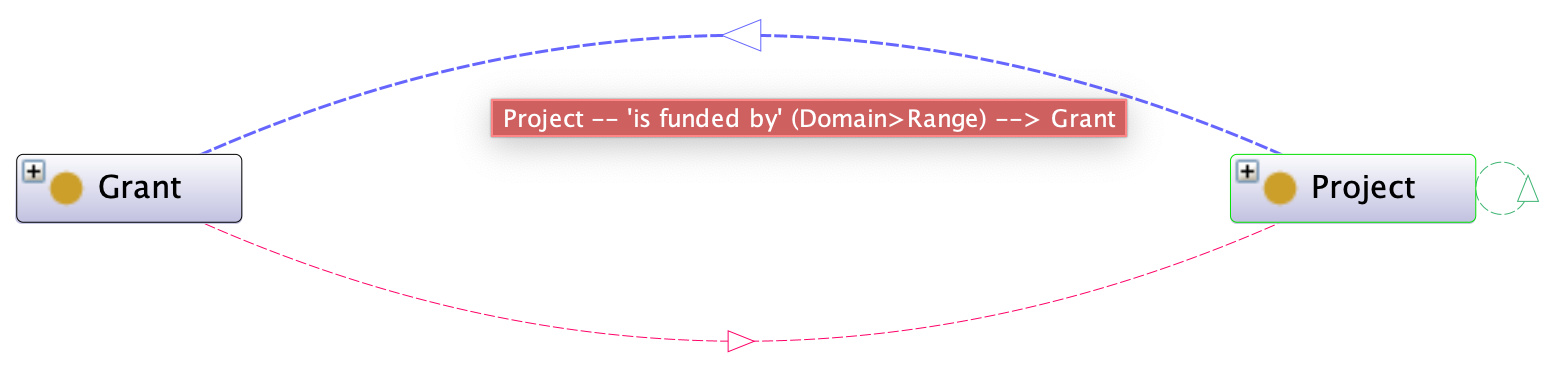
\includegraphics[width=\textwidth]{03_Figures/research-methods/is-funded-by.png}
     \rule{35em}{0.5pt}
    \caption{The \textbf{is funded by} relationship between a project and its grant}
 \label{fig:is-funded-by}
\end{figure}

The ontology also defines relationships between classes, such as \textbf{is funded by}, the association between a project and its grant.
Another example or relationship is \textbf{is employed by}, which links a person, in particular a \textbf{Person Role} to an \text{Organisation}.
The ontology also provides object property descrptions, for example the \textbf{has involved party} relationship, which links a \textbf{Project} to a \textbf{Role}, is inverse of \textbf{is involved in}, which links a \textbf{Role} to a \textbf{Project}.

\begin{figure}[htbp]
    \centering
 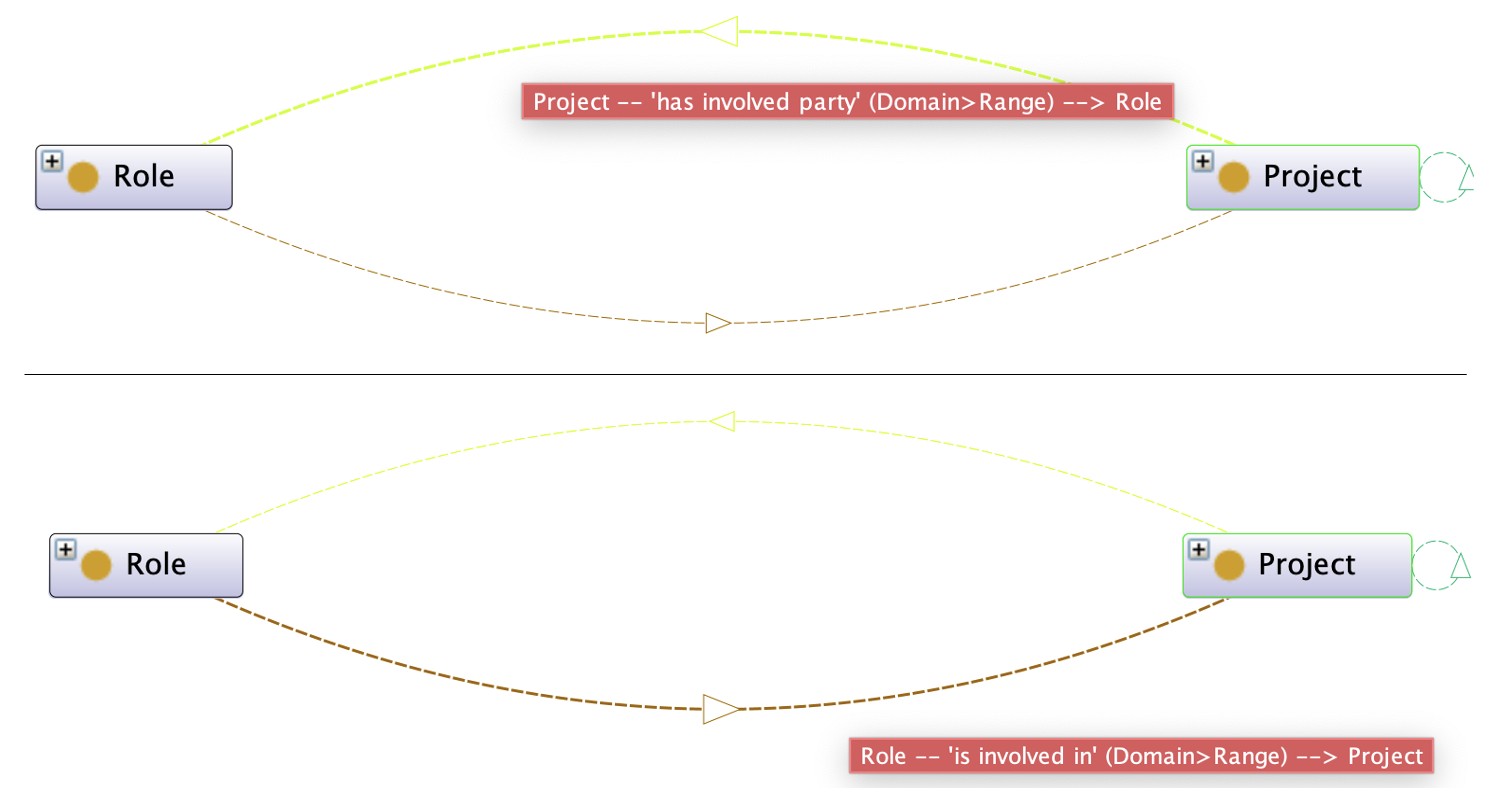
\includegraphics[width=\textwidth]{03_Figures/research-methods/has-involved-party-is-involved-in.png}
     \rule{35em}{0.5pt}
    \caption{The \textbf{has involved party} and \textbf{is involved in} relationships}
 \label{fig:is-involved-in-has-involved-party}
\end{figure}

This object property descriptions can be very useful for querying the \gls{kg} to extract relevant information in a structured manner.
Moreover, the ontology defines a hierarchy of classes.
For example, the \textbf{Organisation} class is a superclass of several subclasses such as \textbf{For Profit Organisation}, \textbf{Funding Agency}, \textbf{Higher Or Secondary Education}, \textbf{Research Organisation}, and \textbf{SME} (Small and Medium Enterprise).

\begin{figure}[htbp]
    \centering
 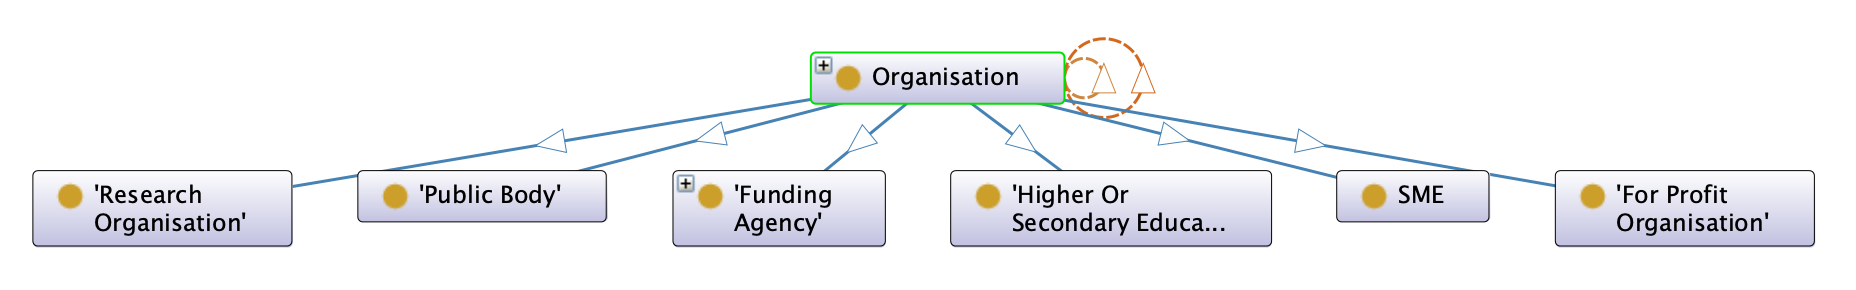
\includegraphics[width=\textwidth]{03_Figures/research-methods/organisation-class-hierarchy.png}
     \rule{35em}{0.5pt}
    \caption{The \textbf{Organisation} class hierarchy}
 \label{fig:organisation-class-hierarchy}
\end{figure}

An overview of the \gls{eurio} ontology is shown in the UML diagram in Fig.~\ref{fig:eurio-ontology}.

\begin{figure}[htbp]
    \centering
 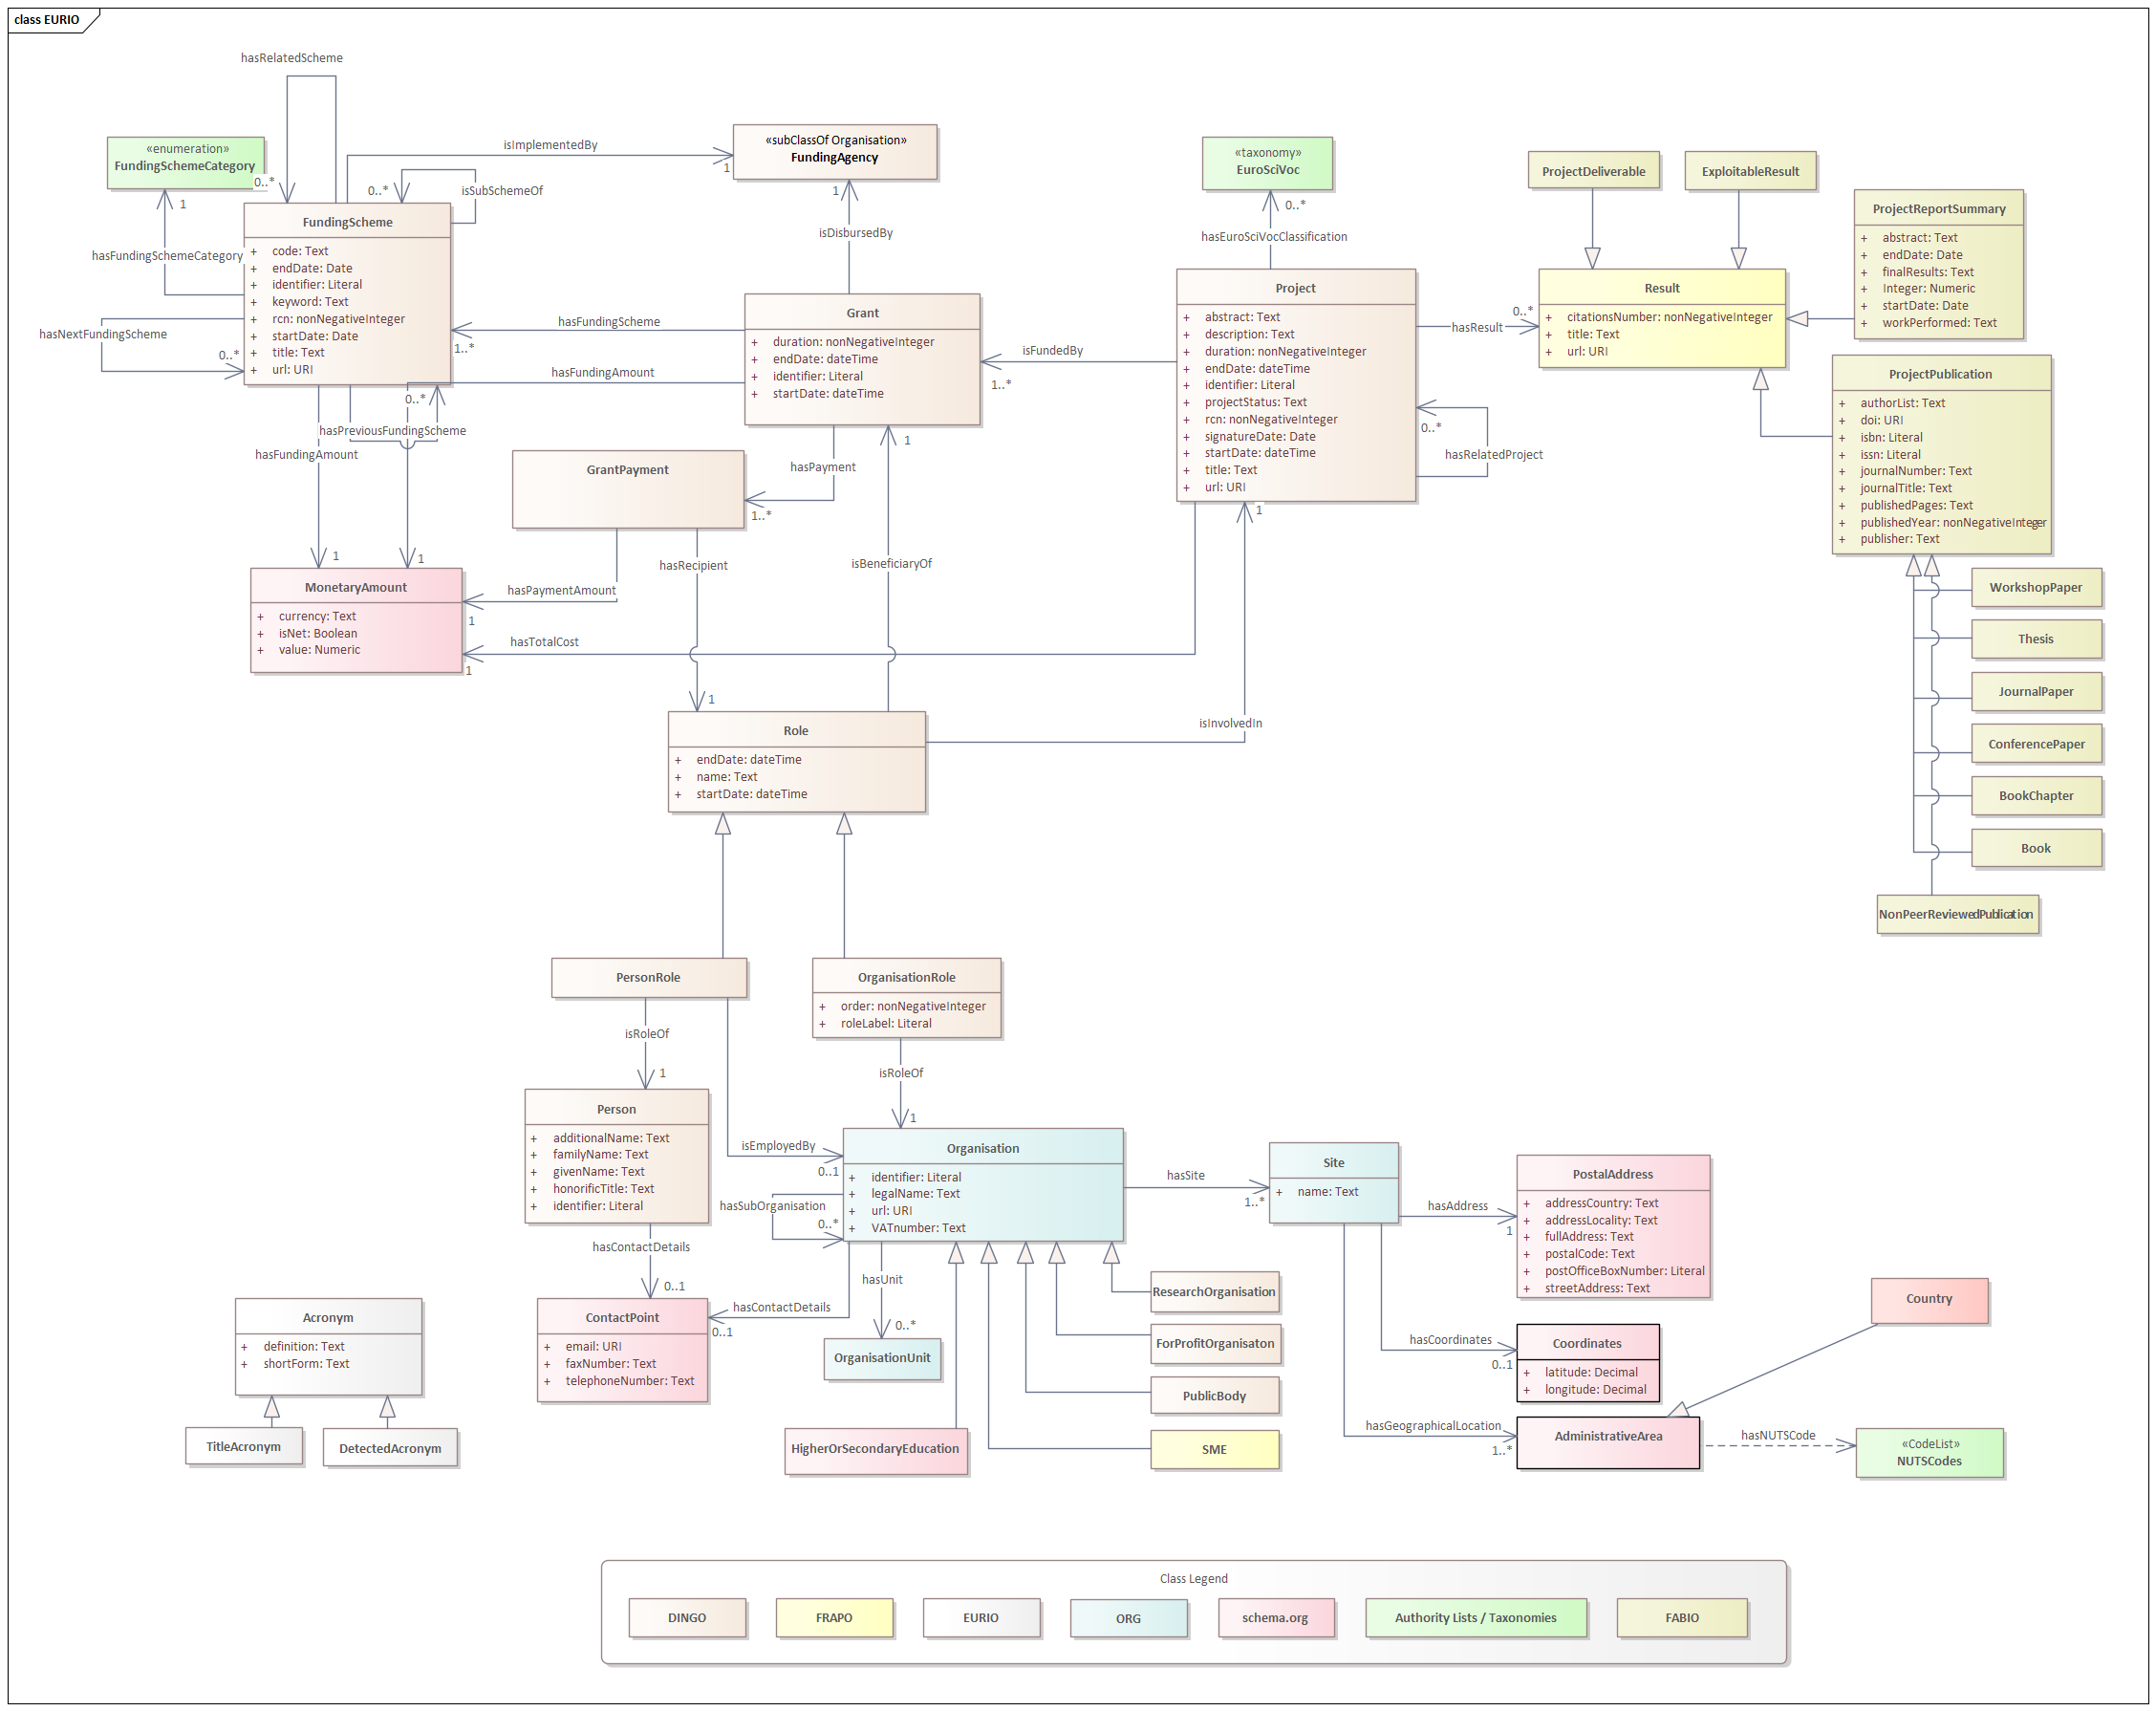
\includegraphics[width=\textwidth]{03_Figures/research-methods/EURIO_V2.4.png}
     \rule{35em}{0.5pt}
    \caption{A graphical representation of the \gls{eurio} ontology (from \url{https://op.europa.eu/en/web/eu-vocabularies/eurio})}
 \label{fig:eurio-ontology}
\end{figure}

\subsection*{Data Availability and Formats}

The \gls{eurio} dataset is available in multiple formats to ensure accessibility and ease of integration into different research workflows.
Supported formats include \gls{rdf}, \gls{ttl}, \gls{nq}, \gls{jsonld}, and \gls{nt}.